\section{Implementando regresiones lineales con \texttt{Python}}

Avancemos y tratemos de hacer un modelo de regresión lineal simple y veamos cuales son los Problemas que encaramos, y como pueden ser resueltos para hacer el modelo más robusto.



Usaremos los datos de publicidad que usamos anteriormente.


Los siguientes dos métodos implementan regresiones lineales en \texttt{Python}:
\begin{itemize}
	\item El método \texttt{ols} (``ordinary least squares'') y la librería \texttt{statsmodel.formula.api}
	\item El paquete \texttt{scikit-learn}
\end{itemize}
Implementemos una regresión lineal simple usando el primer método y después construyamos sobre un modelo de regresión lineal múltiple. Después también nos fijaremos como es que el segundo método es usado para hacer lo mismo.

\subsection{Regresiones lineales usando \texttt{statsmodel}}
[]{statsModelExample.py}
Primero importemos los datos desde \texttt{Advertising.csv}:
\begin{lstlisting}[language=Python]
	import pandas as pd
	advert=pd.read_csv('./dataBases/Advertising.csv')
	print(advert.head())
\end{lstlisting}



Recordemos que esta base de satos contiene información de presupuestos de publicidad gastados en TV, radio y periódicos, para ciertos productos en particular y sus ventas resultantes.


Esperamos una correlación positiva entre tales costos de publicidad y las ventas. Ya hemos visto que existe una buena correlación entre costos de publicidad en TV y ventas.

[]{}
Ahora averigüemos como es esta relación con el siguiente código
\begin{lstlisting}[language=Python]
	import statsmodels.formula.api as smf
	model1=smf.ols(formula='Sales~TV',data=advert).fit()
	print(model1.params)
\end{lstlisting}
del cual obtenemos la siguiente información
\begin{lstlisting}[language=Python]
	Intercept    7.032594
	TV           0.047537
	dtype: float64
\end{lstlisting}



Aquí hemos supuestos que existe una regresión lineal entre costos de publicidad en TV y ventas, y hemos creado el mejor ajuste usando el método de mínimos cuadrados. Entonces, con nuestra notación, esto quiere decir que los parámetros de la regresión lineal tenemos que
\begin{align}
	\a = 7.032594, \; \beta= 0.047537
\end{align}
y la ecuación de nuestro modelo será
\begin{align}
	\texttt{Ventas} = 7.032 + 0.047*\texttt{TV}
\end{align}


Si recuerdas, hemos aprendido que los valores de estos parámetros son estimados y existirán valores$-p$ asociados a estos. \emph{Si los valores$-p$ son muy pequeños, podemos aceptar que tales parámetros tienen un valor diferente de cero y son estadísticamente significativos en el modelo.}

[]
Miremos estos valores $p$ para dichos parámetros
\begin{lstlisting}[language=Python]
	print(model1.pvalues)
	
	Intercept    1.406300e-35
	TV           1.467390e-42
	dtype: float64
\end{lstlisting}

Como puede apreciarse, los valores$-p$ son muy pequeños; por tanto, los parámetros son significativos.

[]{}
Revisemos ahora otro indicador importante de la eficacia del modelo, $R^{2}.$ Aunque nosotros lo implementamos manualmente, podemos obtenerlos con la siguiente línea de código:
\begin{lstlisting}[language=Python]
	print(model1.rsquared)
	
	0.61187505085
\end{lstlisting}


[]{}
Si requerimos todos los parámetros del modelo en un sólo paso, podemos ocupar la siguiente línea de código
\begin{lstlisting}[language=Python]
	print(model1.summary())
\end{lstlisting}
De lo cuál obtenemos

[]
\begin{lstlisting}[language=Python]
	OLS Regression Results
	==============================================================================
	Dep. Variable:                  Sales   R-squared:                       0.612
	Model:                            OLS   Adj. R-squared:                  0.610
	Method:                 Least Squares   F-statistic:                     312.1
	Date:                Sun, 29 Oct 2017   problema (F-statistic):           1.47e-42
	Time:                        04:11:12   Log-Likelihood:                -519.05
	No. Observations:                 200   AIC:                             1042.
	Df Residuals:                     198   BIC:                             1049.
	Df Model:                           1
	Covariance Type:            nonrobust
	==============================================================================
	coef    std err          t      P>|t|      [0.025      0.975]
	------------------------------------------------------------------------------
	Intercept      7.0326      0.458     15.360      0.000       6.130       7.935
	TV             0.0475      0.003     17.668      0.000       0.042       0.053
	==============================================================================
	Omnibus:                        0.531   Durbin-Watson:                   1.935
	problema(Omnibus):                  0.767   Jarque-Bera (JB):                0.669
	Skew:                          -0.089   problema(JB):                        0.716
	Kurtosis:                       2.779   Cond. No.                         338.
\end{lstlisting}



Como podemos ver, el estadístico$-F$ para este modelo es muy alto y el respectivo valor$-p$ es despreciable, lo cual sugiere que los estimados del parámetro para este modelo son todos significativos y no nulos.

[]{}
Ahora predigamos el valor de las ventas basados en la ecuación que acabamos de encontrar. Esto podemos hacer de la siguiente manera
\begin{lstlisting}[language=Python]
	sales_pred=model1.predict(pd.DataFrame(advert['TV']))
	print(sales_pred.head())
	
	0    17.970775
	1     9.147974
	2     7.850224
	3    14.234395
	4    15.627218
	dtype: float64
\end{lstlisting}



Esta ecuación básicamente calcula el valor de las ventas predichas para cada fila basada en la ecuación del modelo usando los costos de \texttt{TV}.

[]{}
Podemos trazar \texttt{sales\_pred} contra el costo de publicidad en \texttt{TV} para encontrar la línea que mejor ajusta:
\begin{lstlisting}[language=Python]
	import matplotlib.pyplot as plt
	advert.plot(kind='scatter', x='TV', y='Sales')
	plt.plot(pd.DataFrame(advert['TV']),sales_pred,c='red',linewidth=2)
	plt.show()
\end{lstlisting}



\begin{center}
	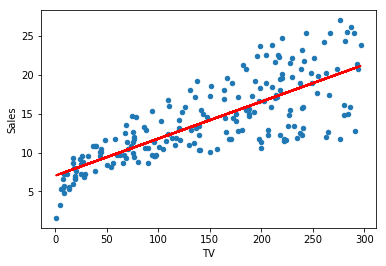
\includegraphics[width=10cm,keepaspectratio=true]{./images/statsModelExample.png}
	% statsModelExample.png: 0x0 pixel, 300dpi, 0.00x0.00 cm, bb=
\end{center}


[]
Ahora calculemos el valor \texttt{RSE}
\begin{lstlisting}[language=Python]
	advert['sales_pred']=0.047537*advert['TV']+7.03
	advert['RSE']=(advert['Sales']-advert['sales_pred'])**2
	SSD=advert.sum()['RSE']
	n = len(advert["Sales"])
	RSE=np.sqrt(SSD/(n-2))
	salesmean=np.mean(advert['Sales'])
	error=RSE/salesmean
	print(RSE,salesmean,error)
\end{lstlisting}


La salida consta de tres números, el primero de los cuales es $\texttt{RSE} = 3.25$, el segundo es
\texttt{salesmean} (media de ventas reales) $= 14.02$ y \texttt{error} es su proporción, que es igual
a $0.23$.




Por lo tanto, en promedio, este modelo tendrá un $23\%$, incluso si los coeficientes son
correctamente predichos.



Esta es una cantidad significativa de errores y nos gustaría bajarla de alguna manera. Además, se puede mejorar el valor de $R^{2}=0.61$.



Algo que
podemos intentar es agregar más columnas en el modelo, como predictores y ver si mejora el resultado o no.

